\documentclass{article}

\setlength{\headsep}{0.75 in}
\setlength{\parindent}{0 in}
\setlength{\parskip}{0.1 in}

%=====================================================
% Add PACKAGES Here (You typically would not need to):
%=====================================================

\usepackage{xcolor}
\usepackage[margin=1in]{geometry}
\usepackage{amsmath,amsthm}
\usepackage{fancyhdr}
\usepackage{enumitem}
\usepackage{graphicx}
\usepackage{amsmath, amssymb}  % Include the amsmath and amssymb packages for mathematical symbols

%=====================================================
% Ignore This Part (But Do NOT Delete It:)
%=====================================================

\theoremstyle{definition}
\newtheorem{problem}{Problem}
\newtheorem*{fun}{Fun with Algorithms}
\newtheorem*{challenge}{Challenge Yourself}
\def\fline{\rule{0.75\linewidth}{0.5pt}}
\newcommand{\finishline}{\begin{center}\fline\end{center}}
\newtheorem*{solution*}{Solution}
\newenvironment{solution}{\begin{solution*}}{{\finishline} \end{solution*}}
\newcommand{\grade}[1]{\hfill{\textbf{($\mathbf{#1}$ points)}}}
\newcommand{\thisdate}{April 25, 2024}
\newcommand{\thissemester}{\textbf{Rutgers: Spring 2024}}
\newcommand{\thiscourse}{ECE 509: Convex Optimization} 
\newcommand{\thishomework}{Number} 
\newcommand{\thisname}{Name} 
\newcommand{\thisextension}{Yes/No} 

\headheight 40pt              
\headsep 10pt
\renewcommand{\headrulewidth}{0pt}
\pagestyle{fancy}

\newcommand{\thisheading}{
   \noindent
   \begin{center}
   \framebox{
      \vbox{\vspace{2mm}
    \hbox to 6.28in { \textbf{\thiscourse \hfill \thissemester} }
       \vspace{4mm}
       \hbox to 6.28in { {\Large \hfill Homework \#\thishomework \hfill} }
       \vspace{2mm}
         \hbox to 6.28in { { \hfill \thisdate  \hfill} }
       \vspace{2mm}
       \hbox to 6.28in { \emph{Name: \thisname \hfill Extension: \thisextension}}
      \vspace{2mm}}
      }
   \end{center}
   \bigskip
}

%=====================================================
% Some useful MACROS (you can define your own in the same exact way also)
%=====================================================


\newcommand{\ceil}[1]{{\left\lceil{#1}\right\rceil}}
\newcommand{\floor}[1]{{\left\lfloor{#1}\right\rfloor}}
\newcommand{\prob}[1]{\Pr\paren{#1}}
\newcommand{\expect}[1]{\Exp\bracket{#1}}
\newcommand{\var}[1]{\textnormal{Var}\bracket{#1}}
\newcommand{\set}[1]{\ensuremath{\left\{ #1 \right\}}}
\newcommand{\poly}{\mbox{\rm poly}}


%=====================================================
% Fill Out This Part With Your Own Information:
%=====================================================


\renewcommand{\thishomework}{8} %Homework number
\renewcommand{\thisname}{Ravi Raghavan} % Enter your name here
\renewcommand{\thisextension}{No} % Pick only one of the two options accordingly

\begin{document}

\thisheading
\vspace{-0.75cm}


%=====================================================
% LaTeX Tip: You can erase this part from here.... 
%=====================================================		

\finishline

%=====================================================
% LaTeX Tip: ... to here
%=====================================================	


\bigskip
\begin{problem} Problem 3.20
\textit{Composition with an affine function.} Show that the following function $f: \mathbb{R}^n \rightarrow \mathbb{R}$ are convex
\begin{itemize}
    \item[(a)] $f(x) = ||Ax - b||$, where $A \in \mathbb{R}^{m x n}$, $b \in \mathbb{R}^m$, and $||.||$ is a norm on $\mathbb{R}^m$
    \begin{solution}
$f(x)$ is a composition of a norm and an affine function. Norms are convex. Hence, since we have a composition with an affine mapping, we have a convex function! 
 
    \end{solution} 

    \item[(b)] $f(x) = - (\det (A_0 + x_1 A_1 + \dots + x_n A_n))^{\frac{1}{m}}$, on $\{x | A_0 + x_1 A_1 + \dots + x_n A_n \succ 0\}$ where $A_i \in \mathbb{S}^m$

    \begin{solution}
    It is clear that $f(x)$ is the composition of $- (\det (X))^{\frac{1}{m}}$ and an affine function(i.e. $A_0 + x_1 A_1 + \dots + x_n A_n$). \newline 

    Now, our goal is to prove that $g(X) = - (\det (X))^{\frac{1}{m}}$, where $X \in \mathbb{S}^m_{++}$ is convex. \newline 

     To verify convexity, we can consider an arbitrary line given by $X = Z + tV$ where $Z \in \mathbb{S}^m_{++}$ and $V \in \mathbb{S}^m$ \newline 

     $h(t) = g(Z + tV) = - (\det (Z + tV))^{\frac{1}{m}}$ \newline 
    $= -(\det (Z^{\frac{1}{2}} (I + tZ^{\frac{-1}{2}} V Z^{\frac{-1}{2}}) Z^{\frac{1}{2}}))^{\frac{1}{m}}$ \newline

    $= - (\det (Z^{\frac{1}{2}}))^{\frac{1}{m}} (\det ((I + tZ^{\frac{-1}{2}} V Z^{\frac{-1}{2}})))^{\frac{1}{m}} (\det (Z^{\frac{1}{2}}))^{\frac{1}{m}}$ \newline

    $= - (\det (Z))^{\frac{1}{m}} (\det ((I + tZ^{\frac{-1}{2}} V Z^{\frac{-1}{2}})))^{\frac{1}{m}}$ \newline

    $= - (\det (Z))^{\frac{1}{m}} (\prod_{i=1}^{m} (1 + t\lambda_i))^{\frac{1}{m}}$ \newline 

    Note: $\lambda_i$ are eigenvalues of $Z^{\frac{-1}{2}} V Z^{\frac{-1}{2}}$ \newline 

     We know that $Z + tV \in \mathbb{S}^m_{++}$ \newline 
    This means that $Z^{\frac{1}{2}} (I + tZ^{\frac{-1}{2}} V Z^{\frac{-1}{2}}) Z^{\frac{1}{2}} \in \mathbb{S}^m_{++}$ \newline 

    For any vector $y$, we know that $y^T Z^{\frac{1}{2}} (I + tZ^{\frac{-1}{2}} V Z^{\frac{-1}{2}}) Z^{\frac{1}{2}} y \geq 0$ \newline 

    We know that $Z^{\frac{1}{2}}$ is symmetric and positive definite. \newline 

    $y^T (Z^{\frac{1}{2}})^T (I + tZ^{\frac{-1}{2}} V Z^{\frac{-1}{2}}) Z^{\frac{1}{2}} y \geq 0$ \newline 

    $(Z^{\frac{1}{2}} y)^T (I + tZ^{\frac{-1}{2}} V Z^{\frac{-1}{2}}) (Z^{\frac{1}{2}} y) \geq 0$ \newline 
    
    This means that $(I + tZ^{\frac{-1}{2}} V Z^{\frac{-1}{2}}) \in \mathbb{S}^m_{++}$ must be True

    This means that $1 + t\lambda_i > 0$ must be true for all $i$! 


    Since $(\prod_{i=1}^{m} (1 + t\lambda_i))^{\frac{1}{m}}$ is a geometric mean of positive numbers, it is concave. \newline 

    $= - (\det (Z))^{\frac{1}{m}} (\prod_{i=1}^{m} (1 + t\lambda_i))^{\frac{1}{m}}$ represents a negative value multiplied by a concave function. \newline 
    
    Hence, $h(t) = - (\det (Z))^{\frac{1}{m}} (\prod_{i=1}^{m} (1 + t\lambda_i))^{\frac{1}{m}}$ is convex! \newline 

    This means that $g(X) = -(\det(X))^{\frac{1}{m}}$ is convex. 

    Hence, we have shown that $f(x)$ is the composition of a convex function with an affine function which means that $f(x)$ is convex. 

    \end{solution}
\end{itemize}
\end{problem}

\begin{problem} Problem 3.21
    {Pointwise maximum and supremum.} Show that the following function $f: \mathbb{R}^n \rightarrow \mathbb{R}$ are convex

    \begin{itemize}
        \item[(a)] $f(x) = \max_{i = 1, \dots, k} || A^{(i)}x - b^{(i)}||$, where $A^{(i)} \in \mathbb{R}^{m x n}$, $b^{(i)} \in \mathbb{R}^m$, and $||.||$ is a norm on $\mathbb{R}^m$

        \begin{solution}
            This function is just a pointwise maximum of a bunch of convex functions(this was proved earlier), which are convex. Hence, $f$ is convex. 
        \end{solution}

        \item[(b)] $f(x) = \sum_{i=1}^{r} |x|_{[i]}$ on $\mathbb{R}^n$, where $|x|$ denotes the vector with $|x|_i = |x_i|$ (i.e. $|x|$ is the absolute value $x$, component wise), and $|x|_{[i]}$ is the $i$th largest component of $|x|$.  In other words,  $|x|_{[1]}, |x|_{[2]}, \dots , |x|_{[n]}$ are the absolute values of the components of $x$, sorted in nonincreasing order.

        \begin{solution}
            We can re-express $f(x)$: \newline 

            $f(x) = \max_{i_1, i_2, \dots, i_r} \{|x_{i_1}| + |x_{i_2}| + \dots + |x_{i_r}|\}$ where $i_k \in [1, n] \enspace \forall k \in [1, r]$ \newline 

            $|x_{i_1}| + |x_{i_2}| + \dots + |x_{i_r}|$ is a convex function since it is a non-negative weighted sum of convex functions(i.e. $L_1$ Norm)

            It is clear that $f(x)$ is the pointwise maximum of $\binom{n}{r}$ convex functions. 

            
        \end{solution}
    \end{itemize}
\end{problem}


\begin{problem} Problem 3.22
\textit{Composition rules.} Show that the following functions are convex.

\begin{itemize}
    \item[(a)] $f(x) = -\log(-\log(\sum_{i=1}^{m} e^{a_i^Tx + b_i}))$ on $dom f = \{ x | \sum_{i=1}^{m} e^{a_i^Tx + b_i} < 1\}$. You can use the fact that $\log(\sum_{i=1}^{m} e^{y_i})$ is convex. 

    \begin{solution}
        We can re-express $f(x)$ as follows: \newline 

        $f(x) = h(g(Ax + b))$ where $h(x) = - \log(x)$ and $g(x) = -\log(\sum_{i=1}^{m} e^{y_i})$ and $A$ is a matrix such that each $a_i$ is a row of $A$ and $b$ is a vector such that each $b_i$ is a row of $b$. 

        Let's start by first analyzing $g(Ax + b)$. We know that $g$ is concave. Hence, $g(Ax + b)$ is concave. 

        Since $h(x) = - \log(x)$, $h(x)$ is convex. 

        Since we have $h$ is convex, $\tilde{h}$ is nonincreasing and $g(Ax + b)$ is concave, we have that $f$ is convex. 
    \end{solution}

    \item[(e)] $f(x, t) = -\log(t^p - ||x||^p_p)$ where $p > 1$ and $dom f = \{(x, t) | t > ||x||_p \}$. You can use the fact that $\frac{||x||^p_p}{u^{p - 1}}$ is convex in $(x, u)$ for $u > 0$

    \begin{solution}
        Let's start rewriting $f(x, t)$ \newline 

        $f(x, t) = -\log(t^{p - 1}(t - \frac{||x||^p_p}{t^{p - 1}}))$ \newline 

        $f(x, t) = -\log(t^{p - 1}) - \log((t - \frac{||x||^p_p}{t^{p - 1}}))$

        $f(x, t) = -(p - 1)\log(t) - \log((t - \frac{||x||^p_p}{t^{p - 1}}))$

        The function $-(p - 1)\log(t)$ is convex since $p > 1$(i.e. $p - 1 > 0$) and $-\log(t)$ is convex. Hence, $-(p - 1)\log(t)$ is a non-negative weighted sum of convex functions. \newline 

        Let's look at $- \log((t - \frac{||x||^p_p}{t^{p - 1}}))$. This function is a composition of a non-increasing convex function(i.e. $-\log(x)$) and a concave function(i.e. $(t - \frac{||x||^p_p}{t^{p - 1}})$). 

        Let's briefly explain why $(t - \frac{||x||^p_p}{t^{p - 1}})$ is concave. $\frac{||x||^p_p}{t^{p - 1}}$ is convex. Hence, $-\frac{||x||^p_p}{t^{p - 1}}$ is concave. $t$ can be viewed as an affine map. Hence, $t$ is convex and concave. The sum of 2 concave functions is concave. Hence, $(t + (- \frac{||x||^p_p}{t^{p - 1}})) = (t - \frac{||x||^p_p}{t^{p - 1}})$ is Concave. 

        Hence, $- \log((t - \frac{||x||^p_p}{t^{p - 1}}))$ is convex. 

        Since $-(p - 1)\log(t)$ and $- \log((t - \frac{||x||^p_p}{t^{p - 1}}))$ are both convex, $f(x, t) = -(p - 1)\log(t) - \log((t - \frac{||x||^p_p}{t^{p - 1}}))$ is convex as well since it is the sum of $-(p - 1)\log(t)$ and $- \log((t - \frac{||x||^p_p}{t^{p - 1}}))$
    \end{solution}
\end{itemize}
    
\end{problem}

\begin{problem} Problem 3.23
    \textit{Perspective of a Function.}

    \begin{itemize}
        \item[(a)] Show that for $p > 1$, 
        \begin{equation}
            f(x, t) = \frac{|x_1|^p + \dots + |x_n|^p}{t^{p - 1}} = \frac{||x||_p^p}{t^{p - 1}}
        \end{equation}
        is convex on $\{ (x, t) | t > 0\}$

        \begin{solution}
            $f(x, t)$ is the perspective function of $||x||_p^p$ which is convex. 

            Let's briefly show that $||x||_p^p$ is convex. \newline 
            $g(x) = ||x||_p^p = |x_1|^p + \dots + |x_n|^p$ \newline 

            $\frac{\partial g}{x_k} = p |x_k|^{p - 1} sign(x_k)$

            $\frac{\partial^2 g}{x_k^2} = p(p - 1) |x_k|^{p - 2} > 0$

            $\frac{\partial^2 g}{x_j x_k} =0$ where $j \neq k$

            It is clear that this Hessian is a Diagonal Matrix with all positive entries. Hence, the Hessian is Positive Definite which means that $g(x)$ is convex. 
        \end{solution}
    \end{itemize}
\end{problem}
\newpage
\begin{problem} Problem 3.26
    \begin{itemize}
        \item[(c)] 
        \begin{solution}
            We are given the following fact: \newline 

            $\prod_{i=n - k + 1}^{n} \lambda_i(X) = \inf \{ \prod_{i=1}^{k} (V^T X V)_{ii} | V \in \mathbb{R}^{n x k}, V^TV = I \}$

            Let's analyze $\prod_{i=1}^{k} (V^T X V)_{ii}$ for a given $V$ where $V^TV = I$ \newline 

            $(V^T X V)_{ii} = v_i^T X v_i$ where $v_i$ is the $i$th column of $V$ \newline 

            We also know that $X$ is Symmetric and Positive Definite. Since $X$ is Positive Definite, $(V^T X V)_{ii} > 0$. We also know that $V$ is an orthogonal matrix. Hence, since $X$ is a positive definite and symmetric matrix, $V^TXV$ is a diagonal matrix that is positive definite. \newline 

            Hence, 
            $\log(\prod_{i=n - k + 1}^{n} \lambda_i(X)) = \inf \{ \log(\prod_{i=1}^{k} (V^T X V)_{ii}) | V \in \mathbb{R}^{n x k}, V^TV = I \}$ \newline 

            $\sum_{i=n - k + 1}^{n} \log(\lambda_i(X)) = \inf \{ \log(\prod_{i=1}^{k} (V^T X V)_{ii}) | V \in \mathbb{R}^{n x k}, V^TV = I \}$

            Since $V^TXV$ is a positive definite diagonal matrix, $\log(\prod_{i=1}^{k} (V^T X V)_{ii}) = \log \det(V^T X V)$ which is concave on the space of positive definite matrices 

            Hence, $\sum_{i=n - k + 1}^{n} \log(\lambda_i(X)) = \inf \{ \log(\prod_{i=1}^{k} (V^T X V)_{ii}) | V \in \mathbb{R}^{n x k}, V^TV = I \}$ can be re-expressed as follows: \newline 

            $\sum_{i=n - k + 1}^{n} \log(\lambda_i(X)) = \inf \{ \log \det (V^T X V) | V \in \mathbb{R}^{n x k}, V^TV = I \}$

            This is clearly a pointwise infimum of a bunch of concave functions. Hence, we know that $\sum_{i=n - k + 1}^{n} \log(\lambda_i(X))$ is Concave. 




            
        \end{solution}
    \end{itemize}
\end{problem}

\begin{problem} Problem 3.32
    \textit{Products and ratios of convex functions.} In general the product or ratio of two convex functions is not convex. However, there are some results that apply to functions on $\mathbb{R}$. Prove the following.

    \begin{itemize}
        \item[(a)] If $f$ and $g$ are convex, both nondecreasing (or nonincreasing), and positive functions on an interval, then $fg$ is convex.

        \begin{solution}
            Goal: Prove that $f(x) g(x)$ is convex. \newline 

            First Derivative of $f(x) g(x) = f'(x) g(x) + f(x) g'(x)$ \newline 

            Second Derivative of $f(x) g(x) = f''(x) g(x) + f'(x) g'(x) + f'(x) g'(x) + f(x) g''(x) = f''(x) g(x) + 2f'(x)g'(x) + f(x) g''(x)$

            Since $f$ and $g$ are convex, we know can replace $f''(x)$ and $g''(x)$ with $k_{f''}$ and $k_{g''}$ where $k_{f''} \geq 0$ and $k_{g''} \geq 0$

            Since $f$ and $g$ are both positive functions, we can replace $f(x)$ and $g(x)$ with $k_{f}$ and $k_{g}$ where $k_{f} > 0$ and $k_{g} > 0$

            Let's rewrite our expression for the second derivative \newline 

            $f''(x) g(x) + 2f'(x)g'(x) + f(x) g''(x) = k_{f''} k_{g} + 2f'(x)g'(x) + k_{f} k_{g''}$ \newline 

            If $f$ and $g$ are either both nondecreasing or both non-increasing this means that either $f'(x) \geq 0, g'(x) \geq 0$ or $f'(x) \leq 0, g'(x) \leq 0$. Either way, the product $2f'(x)g'(x) \geq 0$ and we can denote this as $k_2$

            Our expression for the second derivative becomes: \newline 
            $k_{f''} k_{g} + k_2 + k_{f} k_{g''} \geq 0$ \newline

            Breakdown: \newline 
            $k_{f''} k_{g} \geq 0$ \newline 
            $k_2 \geq 0$ \newline 
            $k_{f} k_{g''} \geq 0$ \newline 

            By proving that the second derivative $\geq 0$, we have shown convexity

        \end{solution}
        \item[(b)] If $f, g$ are concave, positive, with one nondecreasing and the other nonincreasing, then $fg$ is concave.

        \begin{solution}
            Goal: Prove that $f(x) g(x)$ is concave. \newline 

            First Derivative of $f(x) g(x) = f'(x) g(x) + f(x) g'(x)$ \newline 

            Second Derivative of $f(x) g(x) = f''(x) g(x) + f'(x) g'(x) + f'(x) g'(x) + f(x) g''(x) = f''(x) g(x) + 2f'(x)g'(x) + f(x) g''(x)$

            Since $f$ and $g$ are concave, we know can replace $f''(x)$ and $g''(x)$ with $k_{f''}$ and $k_{g''}$ where $k_{f''} \leq 0$ and $k_{g''} \leq 0$

            Since $f$ and $g$ are both positive functions, we can replace $f(x)$ and $g(x)$ with $k_{f}$ and $k_{g}$ where $k_{f} > 0$ and $k_{g} > 0$

            If $f$ and $g$ have one of them nondecreasing and the other nonincreasing this means that either $f'(x) \geq 0, g'(x) \leq 0$ or $f'(x) \leq 0, g'(x) \geq 0$. Either way, the product $2f'(x)g'(x) \leq 0$ and we can denote this as $k_2$

            Our expression for the second derivative becomes: \newline 
            $k_{f''} k_{g} + k_2 + k_{f} k_{g''} \leq 0$ \newline

            Breakdown: \newline 
            $k_{f''} k_{g} \leq 0$ \newline 
            $k_2 \leq 0$ \newline 
            $k_{f} k_{g''} \leq 0$ \newline 

            By proving that the second derivative $\leq 0$, we have shown concavity
            

        \end{solution}
        \item[(c)] If $f$ is convex, nondecreasing, and positive, and $g$ is concave, nonincreasing, and positive, then $f /g$ is convex.
        \begin{solution}
            Let's look at $1/g$ \newline 

            First Derivative of $1/g$: $\frac{-g'(x)}{(g(x))^2}$ \newline 

            Second Derivative of $1/g$: $\frac{-g''(x)(g(x))^2 + 2g(x) (g'(x))^2}{(g(x))^4}$ \newline 

            Since $g$ is concave, $g''(x)$ is $\leq 0$. Hence, $-g''(x)(g(x))^2$ is $\geq 0$. Since $g$ is positive, $2g(x) (g'(x))^2$ is $> 0$. 

            Hence, $\frac{-g''(x)(g(x))^2 + 2g(x) (g'(x))^2}{(g(x))^4} \geq 0$

            $1/g$ is convex, nondecreasing, and positive. \newline 

            Since $f$ and $1/g$ are both convex, nondecreasing, and positive, based on Part $(a)$, $f/g$ is convex as well. 

        \end{solution}
    \end{itemize}
\end{problem}

\begin{problem}
    Problem 4.1. Consider the optimization problem 
    \begin{align*}
\text{minimize} \quad & f_0(x_1, x_2) \\
\text{subject to} \quad & 2x_1 + x_2 \geq 1\\
\quad & x_1 + 3x_2 \geq 1\\
& x_1 \geq 0, \enspace x_2 \geq 0
\end{align*}

Make a sketch of the feasible set. For each of the following objective functions, give the optimal set and the optimal value.

\begin{figure}[h!]
        \centering
        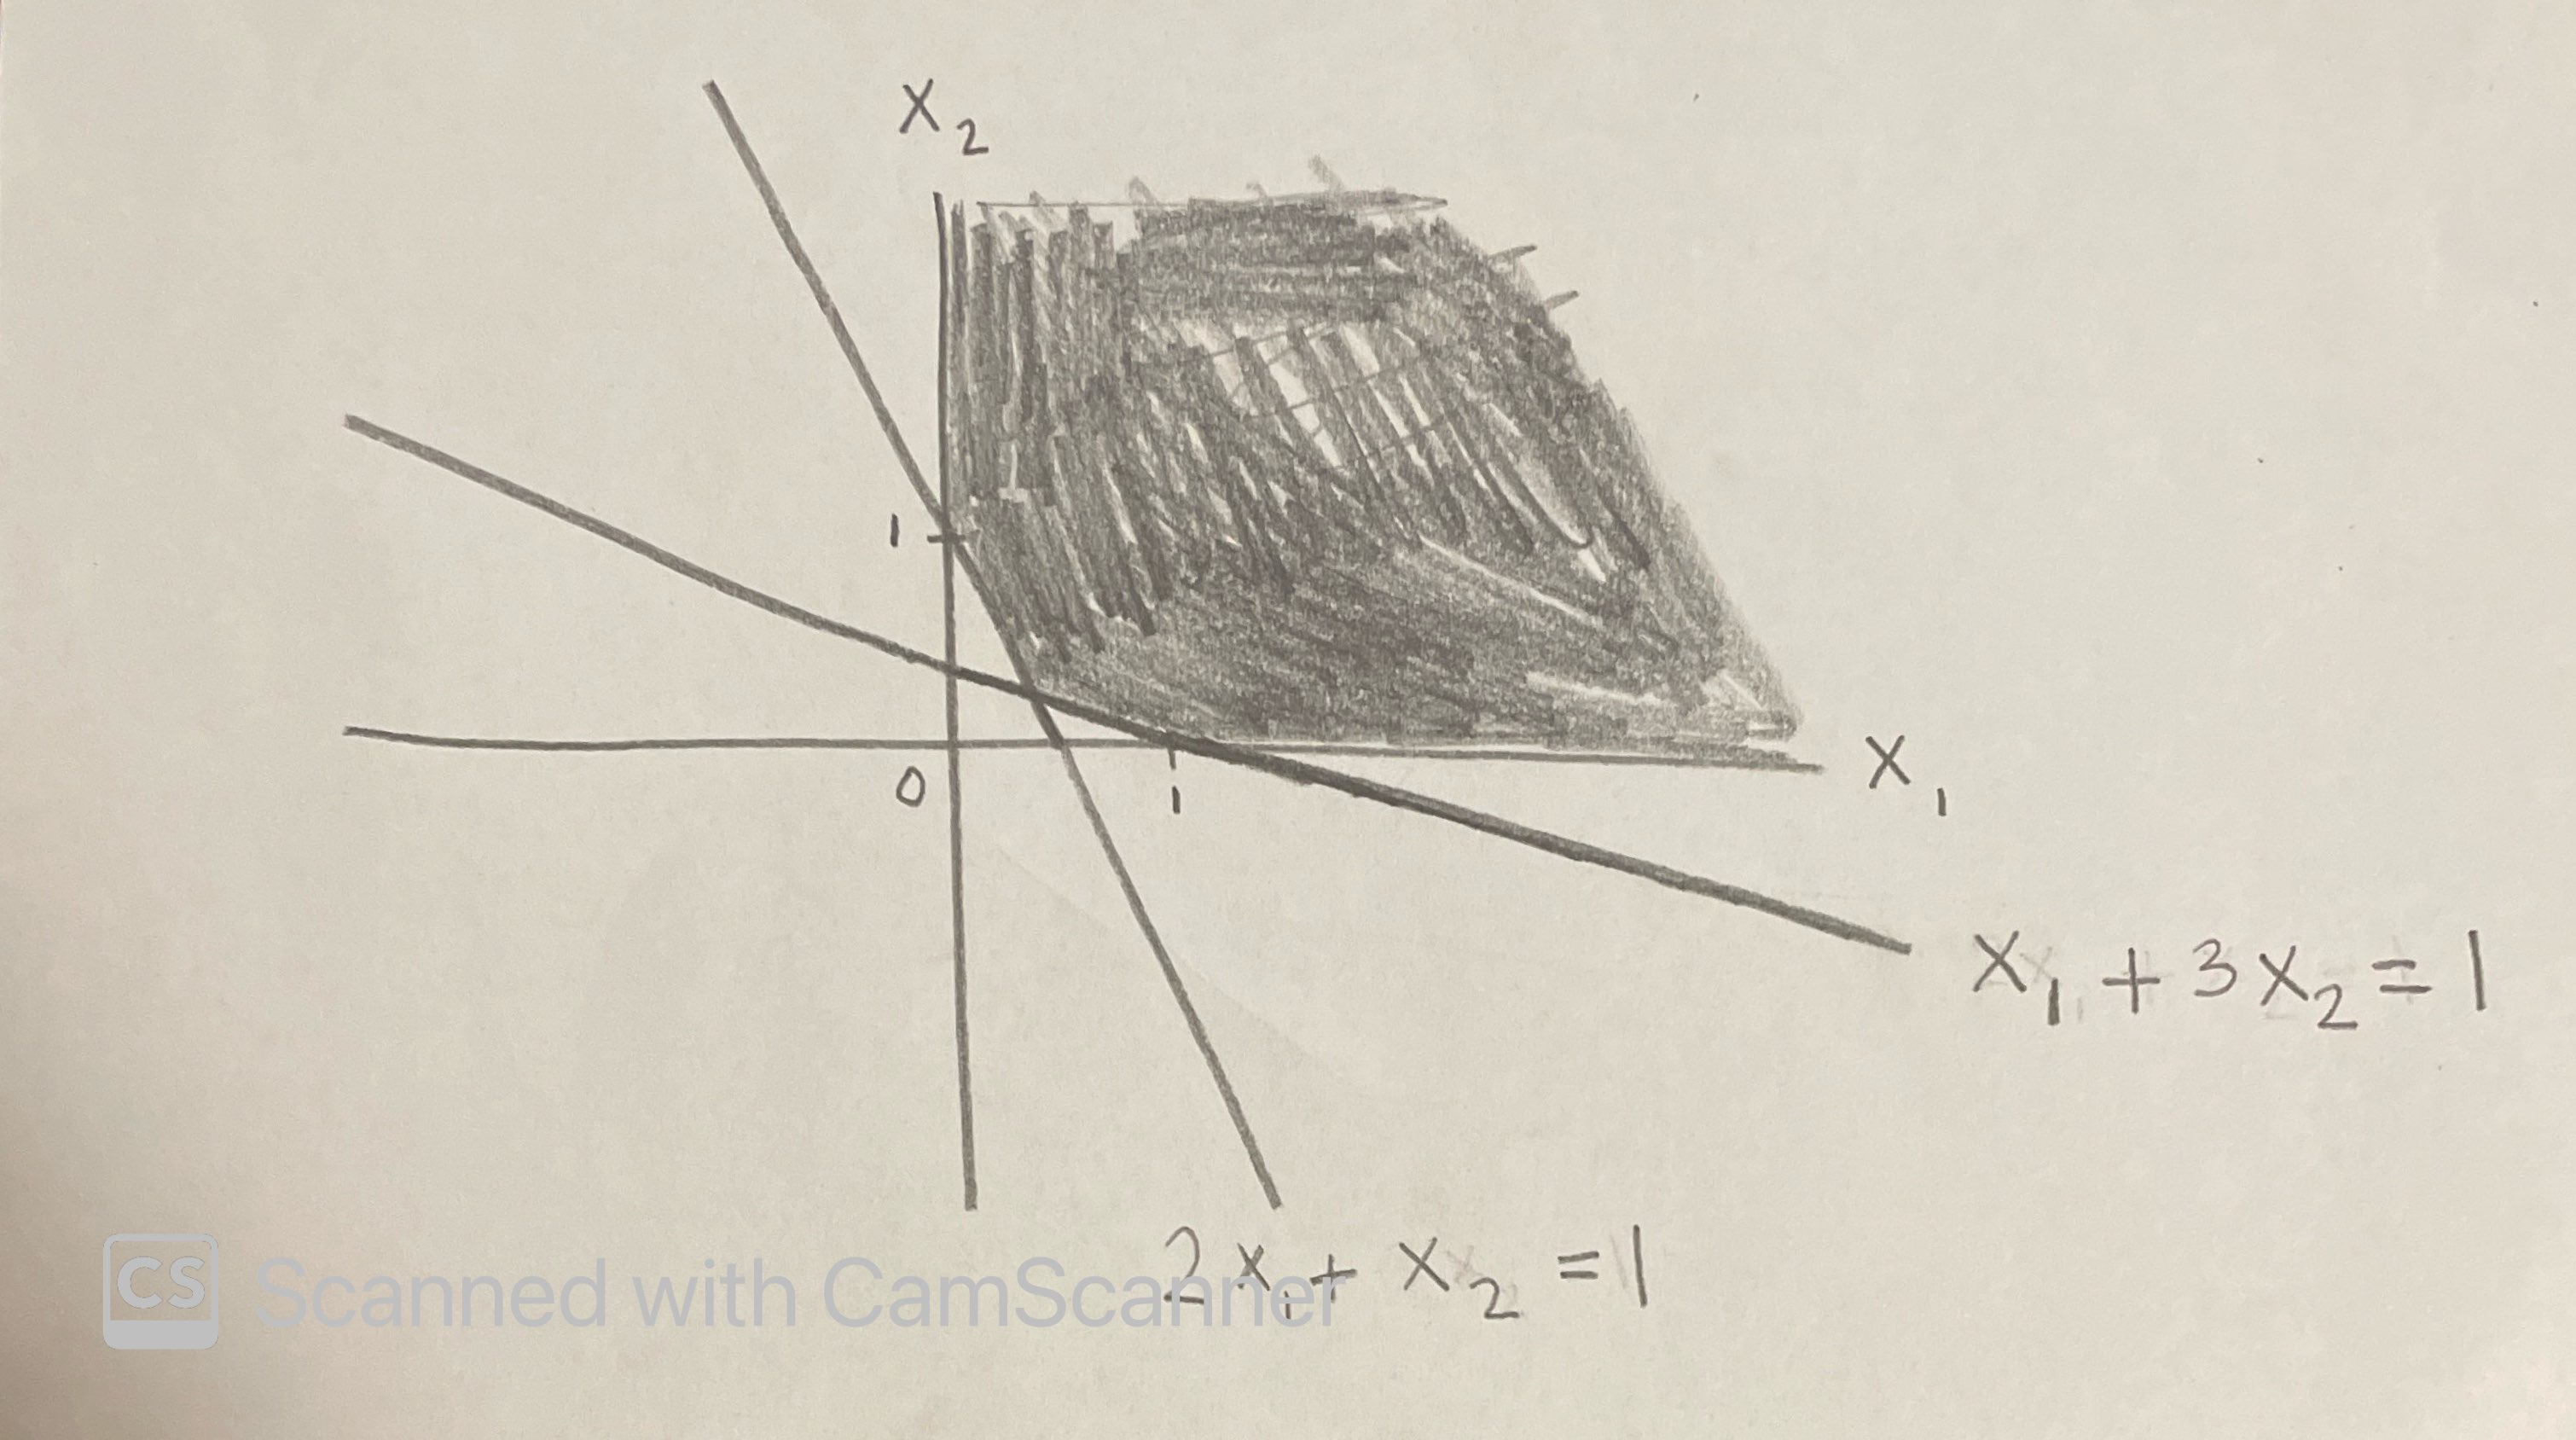
\includegraphics[width=0.6 \textwidth]{HW8-2n_1.jpg}
        \caption{Set of Feasible Set}
    \end{figure}

Note: The feasible set is the convex hull of the following points $(0, 1)$, $(0.4, 0.2)$, $(1, 0)$, $(0, \infty)$, $(\infty, 0)$

\begin{itemize}
    \item[(a)] $f_0(x_1, x_2) = x_1 + x_2$
    \begin{solution}
        Optimal Set: $\{(0.4, 0.2)\}$, Optimal Value: $0.6$
    \end{solution}
    \item[(b)] $f_0(x_1, x_2) = - x_1 - x_2$
    \begin{solution}
        This one is unbounded below. Hence, we can essentially say that Optimal Set: $\{(\infty, \infty)\}$, Optimal Value: $-\infty$
    \end{solution}
    \item[(c)] $f_0(x_1, x_2) = x_1$  
    \begin{solution}
        Optimal Set: $\{(0, x_2) | x_2 \geq 1\}$, Optimal Value: $0$
    \end{solution}
    \item[(d)] $f_0(x_1, x_2) = \max\{x_1, x_2\}$
    \begin{solution}
    The level curve of the objective function, $f_0(x_1, x_2) = \frac{1}{4}$, is tangent to the constraint line $x_1 + 3x_2 = 1$ at $(\frac{1}{4}, \frac{1}{4})$ which yields an objective function value of $\frac{1}{4}$. However, the point $(\frac{1}{4}, \frac{1}{4})$ is outside the feasible set. To see this $2x_1 + x_2 = 0.75 < 1$ \newline 
    
    The level curve of the objective function, $f_0(x_1, x_2) = \frac{1}{3}$, is tangent to the constraint line $2x_1 + x_2 = 1$ at $(\frac{1}{3}, \frac{1}{3})$ which yields an objective function value of $\frac{1}{3}$. This point is inside the feasible set. $2x_1 + x_2 = 1$, $x_1 + 3x_2 > 1$, $x_1 > 0$, $x_2 > 0$ \newline
    
        Optimal Set: $\{(\frac{1}{3}, \frac{1}{3})\}$, Optimal Value: $\frac{1}{3}$
    \end{solution}
    \item[(e)] $f_0(x_1, x_2) = x_1^2 + 9x_2^2$
    \begin{solution}
    Gradient: $\langle 2x_1, 18x_2 \rangle$ \newline 

    We want the gradient to be tangent to either one of the constraint lines $2x_1 + x_2 = 1$ or $x_1 + 3x_2 = 1$. \newline 

    The constraint lines $2x_1 + x_2 = 1$ and $x_1 + 3x_2 = 1$ have slopes $-2$ and $-\frac{1}{3}$ respectively. \newline 

For the gradient to be tangent to $2x_1 + x_2 = 1$, the slope of the gradient has to be $\frac{1}{2}$. This means that $\frac{9x_2}{x_1} = \frac{1}{2}$ which means that $\frac{x_2}{x_1} = \frac{1}{18}$ \newline 


$2x_1 + \frac{x_1}{18} = 1$, which means that $x_1 = \frac{18}{37}, x_2 = \frac{1}{37}$. This point is NOT inside the feasible set. $x_1 + 3x_2 < 1$ \newline 

For the gradient to be tangent to $x_1 + 3x_2 = 1$, the slope of the gradient has to be $3$. This means that $\frac{9x_2}{x_1} = 3$ which means that $\frac{x_2}{x_1} = \frac{1}{3}$ \newline 


$x_1 + x_1 = 1$, which means that $x_1 = \frac{1}{2}, x_2 = \frac{1}{6}$. This point is inside the feasible set. $x_1 + 3x_2 = 1$, $2x_1 + x_2 > 1$, $x_1 > 0$, $x_2 > 0$.  Overall, this would mean that $f_0(x_1, x_2) = \frac{1}{2}$ \newline 
    
        Optimal Set: $\{(\frac{1}{2}, \frac{1}{6})\}$, Optimal Value: $0.5$
    \end{solution}
\end{itemize}
\end{problem}

\begin{problem}
    Problem 4.3. Prove that $x^* = (1, \frac{1}{2}, -1)$ is optimal for the optimization problem

    \begin{align*}
\text{minimize} \quad & (1/2)x^TPx + q^Tx + r \\
\text{subject to} \quad & -1 \leq x_i \leq 1, \quad i = 1, 2, 3\\
\end{align*}

where:
\begin{itemize}
    \item $P = \begin{bmatrix}
13 & 12 & -2 \\
12 & 17 & 6 \\
-2 & 6 & 12
\end{bmatrix}$, $q = \begin{bmatrix}
-22.0\\
-14.5\\
13.0
\end{bmatrix}$, $r = 1$
\end{itemize}

\begin{solution}
    The optimality condition is that $\nabla f(x^*) (y - x^*) \geq 0$

    $\nabla f(x) = Px + q$ \newline 
    $\nabla f(x^*) = (-1, 0, 2)$

Substituting this back into the optimality condition means that: \newline 
$-1 (y_1 - 1) + 2 (y_3 + 1) \geq 0$

$-1(y_1 - 1) \geq 0$ is always True given that $-1 \leq y_i \leq 1$.  \newline 
$2 (y_3 + 1) \geq 0$ is always True given that $-1 \leq y_i \leq 1$. 

Hence, we know that $-1 (y_1 - 1) + 2 (y_3 + 1) \geq 0$ is ALWAYS true meaning that $x^*$ is optimal!
    
\end{solution}
\end{problem}

\begin{problem} Problem 4.5
    \textit{Equivalent convex problems.} Show that the following three convex problems are equivalent. Carefully explain how the solution of each problem is obtained from the solution of the other problems. The problem data are the matrix $A \in \mathbb{R}^{m x n}$(with rows $a_i^T$), the vector $b \in \mathbb{R}^m$, and the constant $M > 0$.
    \begin{itemize}
        \item[(a)] The \textit{robust least-squares problem}
        \begin{align*}
\text{minimize} \quad & \sum_{i=1}^{m} \phi(a_i^T x - b_i), \\
\end{align*}
with variable $x \in \mathbb{R}^n$, where $\phi: \mathbb{R} \rightarrow \mathbb{R}$ is defined as 
\begin{equation}
    \phi(u) = \begin{cases} 
      u^2 & \text{if } |u| \leq M \\
      M(2|u| - M) & \text{if } |u| > M 
   \end{cases}
\end{equation}

        \item[(b)] The \textit{least-squares problem with variable weights}
 \begin{align*}
\text{minimize} \quad & \sum_{i=1}^{m} (a_i^T x - b_i)^2/(w_i + 1) + M^2\textbf{1}^Tw \\
\text{subject to} \quad & w \succeq 0,\\
\end{align*}
with variables $x \in \mathbb{R}^n$ and $w \in \mathbb{R}^m$, and domain $\mathbb{D} = \{(x, w) \in \mathbb{R}^n \times \mathbb{R}^m | w \succ \textbf{-1} \}$

        \item[(c)] The \textit{quadratic program}
        \begin{align*}
\text{minimize} \quad & \sum_{i=1}^{m} (u_i^2 + 2Mv_i) \\
\text{subject to} \quad & -u - v \preceq Ax - b \preceq u + v\\
\quad & 0 \preceq u \preceq M\textbf{1}\\
& v \succeq 0
\end{align*}
    \end{itemize}

\begin{solution}

Step 1: Show that Problems $(a)$ and $(b)$ are Equivalent: \newline 
Let's work with the objective function of Problem $(b)$ \newline 

$g(w) = \sum_{i=1}^{m} (a_i^T x - b_i)^2/(w_i + 1) + M^2\textbf{1}^Tw$ \newline 

$g(w) = \sum_{i=1}^{m} (a_i^T x - b_i)^2/(w_i + 1) + M^2(\sum_{i=1}^{m} w_i)$ \newline 

If we fix $A$, $b$, $M$, and $x$, we can show that this is a convex function with respect to $w$ \newline

$\frac{\partial g}{\partial w_i} = \frac{-(a_i^T x - b_i)^2}{(w_i + 1)^2} + M^2$ \newline

$\frac{\partial^2g}{\partial w_i \partial w_j} = 0$ when $i \neq j$ \newline
$\frac{\partial^2g}{\partial w_i \partial w_j} = \frac{2(a_i^T x - b_i)^2}{(w_i + 1)^3}$ when $i = j$ \newline

The Hessian is clearly a diagonal matrix whose elements are positive due to the fact that $w \succeq 0$. Hence, on $w \succeq 0$, $g$ is convex. 

To set its gradient to 0, we see that $\frac{-(a_i^T x - b_i)^2}{(w_i + 1)^2} + M^2 = 0$

This means that $(w_i + 1)^2 = \frac{(a_i^T x - b_i)^2}{M^2}$ \newline 

$(w_i + 1) = \frac{|(a_i^T x - b_i)|}{M}$ \newline 

However, due to the restriction that $w \succeq 0$ we must modify this: \newline

$w_i = \begin{cases} 
      \frac{|(a_i^T x - b_i)|}{M} - 1 & \text{if } \frac{|(a_i^T x - b_i)|}{M} \geq 1 \\
      0 & \text{if } \frac{|(a_i^T x - b_i)|}{M} < 1 
   \end{cases}$

$w_i = \begin{cases} 
      \frac{|(a_i^T x - b_i)|}{M} - 1 & \text{if } |(a_i^T x - b_i)| \geq M \\
      0 & \text{if } |(a_i^T x - b_i)| < M
   \end{cases}$

Substituting this into the objective function, we see that: \newline 

$g = \sum_{i=1}^{m} (a_i^T x - b_i)^2/(w_i + 1) + M^2(\sum_{i=1}^{m} w_i)$ \newline 

$g = \sum_{i=1}^{m} (a_i^T x - b_i)^2/(w_i + 1) + \sum_{i=1}^{m} M^2 w_i$ \newline 

$g = \sum_{i=1}^{m} \begin{cases} 
      M|(a_i^T x - b_i)| + M|(a_i^T x - b_i)| - M^2  & \text{if }  |(a_i^T x - b_i)| \geq M \\
      (a_i^T x - b_i)^2 & \text{if } |(a_i^T x - b_i)| < M
   \end{cases}$ \newline 

$g = \sum_{i=1}^{m} \begin{cases} 
      2M|(a_i^T x - b_i)| - M^2  & \text{if }  |(a_i^T x - b_i)| \geq M \\
      (a_i^T x - b_i)^2 & \text{if } |(a_i^T x - b_i)| < M
   \end{cases}$ \newline 

$g = \sum_{i=1}^{m} \begin{cases} 
      M(2|(a_i^T x - b_i)| - M)  & \text{if }  |(a_i^T x - b_i)| \geq M \\
      (a_i^T x - b_i)^2 & \text{if } |(a_i^T x - b_i)| < M
   \end{cases}$ \newline 

$g = \sum_{i=1}^{m} \phi(a_i^T x - b_i)$ \newline 

Step 2: Show that Problems $(a)$ and $(c)$ are Equivalent: \newline 

    The constraints of Problem $(c)$ are that $u_i + v_i \geq |a_i^T x - b_i|$ and that $0 \leq u_i \leq M$ and that $0 \leq v_i$. Clearly, we want $u_i + v_i = |a_i^T x - b_i|$ because if $u_i + v_i > |a_i^T x - b_i|$, with $0 \leq u_i \leq M$ and that $0 \leq v_i$, then we can lower either $u_i$ or $v_i$ and lower the objective function while still meeting the constraints. 

    $u_i + v_i = |a_i^T x - b_i|$, $v_i = |a_i^T x - b_i| - u_i$

Let's work with the objective function for Problem (c). \newline 

Objective function: $g(u) = \sum_{i=1}^{m} u_i^2 + 2Mv_i$ \newline 

Lets substitute the value of $v_i$ into the objective function \newline


    Objective function: $g(u) = \sum_{i=1}^{m} u_i^2 + 2M|a_i^T x - b_i| - 2Mu_i$ \newline

    This is clearly convex with respect to $u$ \newline 

    $\frac{\partial g}{\partial u_i} = 2u_i - 2M$

    $\frac{\partial^2 g}{\partial u_i \partial u_j} = 0$ when $i \neq j$ \newline 
    $\frac{\partial^2 g}{\partial u_i \partial u_j} = 2$ when $i = j$

    The Hessian is clearly a diagonal matrix whose elements are positive Hence, $g$ is convex with respect to $u$. 

    Setting the gradient to 0 implies that $u_i = M$. However, we must be careful. Since $v_i = |a_i^T x - b_i| - u_i$ and $v_i \geq 0$. $u_i = M$ can only happen when $|a_i^T x - b_i| \geq M$. Else, we must set $u_i = |a_i^T x - b_i|$ and $v_i = 0$

    Knowing this we can rewrite our objective function: 

$g = \sum_{i=1}^{m} \begin{cases} 
      M^2 + 2M|a_i^T x - b_i| - 2M^2  & \text{if }  |(a_i^T x - b_i)| \geq M \\
      |a_i^T x - b_i|^2 + 2M|a_i^T x - b_i| - 2M|a_i^T x - b_i| & \text{if } |(a_i^T x - b_i)| < M
   \end{cases}$ \newline 

$g = \sum_{i=1}^{m} \begin{cases} 
      2M|a_i^T x - b_i| - M^2  & \text{if }  |(a_i^T x - b_i)| \geq M \\
      |a_i^T x - b_i|^2  & \text{if } |(a_i^T x - b_i)| < M
   \end{cases}$ \newline 

$g = \sum_{i=1}^{m} \begin{cases} 
      M(2|a_i^T x - b_i| - M)  & \text{if }  |(a_i^T x - b_i)| \geq M \\
      |a_i^T x - b_i|^2  & \text{if } |(a_i^T x - b_i)| < M
   \end{cases}$ \newline 

$g = \sum_{i=1}^{m} \phi(a_i^T x - b_i)$ \newline 

\end{solution}
\end{problem}

\end{document}





